Two dimensional Images, or textures, mapped to three dimensional objects have long been used to efficiently add pre-calculated detail to a 3D scene in computer graphics. In the past decade however, procedural textures has gained an increasing amount of traction as a serious contender to the traditional bitmap texture. The procedural approach presents a new way of generating textures mathematically with a high level of editability, arbitrary levels of detail, compactness and seamless transition between object faces, see figure \ref{fig:BitmapVsProcedural}. With programs such as Blender or Substances Designer growing in popularity and even being adopted by industry professionals, tools for creating procedural texture models using node graph editors are now more accessible than ever \cite{blenderfoundation_2020_blenderorg, a2020_substance}. 

Despite its very appealing advantages, procedural textures remain as an advanced alternative to traditional texturing methods for mainly one reason alone; they are difficult to design to achieve desired results. While modern tools present users with a node editor that abstracts away the underlying functions, figuring out how to compose nodes and what values to assign sometimes hundreds of parameters in order to achieve desired results, is very time consuming and convoluted. The recent advances in texture synthesis using neural networks, e.g. \textit{TileGAN}, present an exemplar based alternative that can generate higher quality versions of user example textures, although not solving the problems with seams and compactness of traditional textures \cite{frhstck_2019_tilegan}. Still, this example of an \textit{inverse} modeling process is much simpler to use for a novel user, especially as there already exists a plethora of bitmap images freely available on the web which can serve as a target to such an inverse problem. 

This thesis focuses on an \textit{inverse procedural texture modeling} problem, a research field that aims to inverse the rendering process and estimate parameters of procedural texture models such that the rendered result matches an input image. However, due to the complexity of most modern render engines built without this functionality in mind, the relationship between procedural modern parameters is non-linear and near impossible to differentiate. Additionally, developing a suitable loss function that can measure image similarity is a non trivial task, due to the discrepancy that exists between the way a computer and a human perceive images.

A few fully differentiable rendering engines have already been developed, such as \textit{OpenDR} or \textit{PyTorch3D}, but neither have direct support for procedural textures \cite{loper_2014_opendr, facebookresearch_2020_facebookresearchpytorch3d}. Recently Guo et. al published a paper detailing a framework for procedural parameter estimation using Bayesian inference \cite{guo_2019_a}. Their results are promising and the contribution of suitable loss functions serve as an inspiration for this thesis. However, their framework did not allow the user to compose their own procedural textures and only tested their algorithm on hard-coded procedural models. Noticing a gap in the field of inverse procedural texture modeling, we present DiPTeR, a Differentiable Procedural Texture Renderer that allows users to dynamically build fully differentiable procedural textures and automatically estimate parameters from a target image. 


\begin{figure}
    \centering
    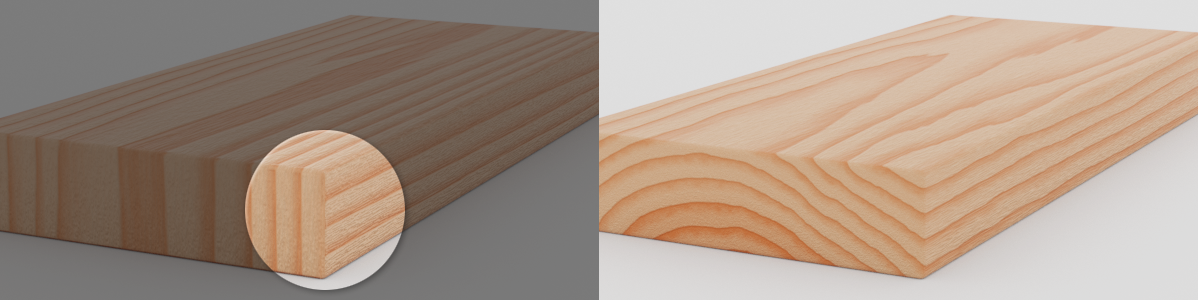
\includegraphics[width=\textwidth]{img/theory/PlaneOrNotAPlane.png}
    \caption{Left$:$ Using a bitmap texture can result in visible seams between object faces as it is inherently difficult to naturally map a 2D texture onto a 3D object. Right$:$ A similar texture rendered with a procedural model. As procedural textures are functions of an objects 3D coordinates, a seamless result is achieved \cite{_comparison}.}
    \label{fig:BitmapVsProcedural}
\end{figure}

\section{Goal}

To alleviate the problems of creating complex procedural texture models by hand, our goal is to develop a \textit{Differentiable Procedural Texture Renderer} or DiPTeR, which can render procedural textures in OpenGL but include a fully differentiable back-end renderer to mimic the rendering process in OpenGL. The back-end renderer should be written in a framework that allows for automatic differentiation, allowing us to create procedural functions and rendering procedures of arbitrary complexity while retaining differentiability. The framework should include a node editor, much like Blender and Substance Designer, that lets users easily build procedural texture models and see their rendered results in real time. A user should be able to present a target bitmap texture, and let the system automatically estimate the optimal parameter values of their procedural texture setup. This means that automatically building a node graph that can render the target image is outside the scope of this project, and is an entirely different problem on its own. Measuring similarity between rendered texture and target texture is done with the means of loss functions, and the framework should allow the user to easily select and implement their own loss functions. While the framework is intended to be operated through a graphical interface developed by us, it should be possible to run the entire texture matching algorithm through a non-graphic user interface.

Through evaluation of our system, we would like to answer the following research questions: Is it possible to build an efficient, differentiable rendering system in PyTorch? Can we achieve an acceptable parameter estimation for a complex procedural texture? Is it fast enough to be usable? Can we find a loss function that performs well in the general case?

\section{Methodology}

Our DiPTeR framework mainly consists of two fairly disconnected parts; the forward user-facing rendering and the backward hidden rendering. The forward rendering is implemented in the popular computer graphics standard OpenGL using python code bindings. All procedural shaders are implemented as fragment shaders written in GLSL, see section \ref{sec:RenderingInOpenGL}. As OpenGL or GLSL doesn't actually have any support for compositing shaders or reusing code, that functionality has been implemented by ourselves, see sections \ref{sec:CompositeShaders} and \ref{sec:ImportPreprocessorDirective} respectively. The backwards rendering is built from scratch in \textit{PyTorch}, a machine learning framework developed by Facebook which includes an automatic differentiation package, As it is a vital component of modern machine learning \cite{paszke_2019_pytorch}. Our backward rendering process is fully differentiable as long as its implemented in the PyTorch ecosystem, and can be used to estimate our forward parameters if implemented to mimic the forward process as closely as possible. One drawback, however, is that PyTorch is not optimized for computer graphics but implementing our procedural shaders as functions of matrices results in adequate performance, and our users will only see the effects of the backwards rendering when running texture matching.

To assists users in designing procedural shaders and see the effects of their choices in real time, we develop a graphical user interface using \textit{PyQt5}, a Python binding for the modern C++ interface library \textit{Qt} \cite{theqtcompany_qt}. Most notibly, we develop a node editor where nodes represent procedural functions that can be composed by connecting nodes' input and output \textbf{REF image?}. We also develop a texture matching interface where a user can select a target image and run our algorithm to automatically estimate parameters of the composed shader function. We use stochastic gradient descent for parameter optimization in our our texture matching algorithm, and PyTorch, being a machine learning framework, proves to be a good choice as it has built in support for Loss functions and Optimizers.

\textbf{Finish with describing evaluation, how data was collected. Did we do user tests? What data was collected?}

\section{Contributions}
\textit{Specify your contributions. What does this particular work/report bring to the research or to the body of knowledge?}

\begin{enumerate}
    \item Using old techniques in new ways = Gradient Descent for inverse rendering. 
    \item Implementing an inverse procedural texture renderer. (even if this is done in pytorch 3d)
    \item Comparison of loss function and optimizers that work best for this task
    \item Ability to easily implement new shaders as well as connecting shaders into compound shaders that are still fully differentiable.
\end{enumerate}

\section{Report outline}

\textbf{Save to last and describe the format and structure of the report.}

% \section{Background}
% \newlist{todolist}{itemize}{2}
% \setlist[todolist]{label=$\square$}
% \begin{todolist}
%     \item Describe why it is not possible to inverse render the existing frameworks, like substance designer or blender!
%     \item Beskriv inverse graphics!
%     \item Mention popular tools that enable use of procedural generation (Blender, 3Ds max, Substance Designer
%     \begin{enumerate}
%         \item Substance designer is popular, but has one large problem in that it only renders to an image. This can be very useful, but isn't tied in to the whole rendering process as well as the other tools, and you can't animate stuffz I think.
%         \item Blender and 3DS max are parts of a whole workflow, but complicated and hard to use. 
%     \end{enumerate}
%     \item[\done]Why are procedural texture hard to work with
%     \item[\done]Why not image synthesis? What is it?
%     \item[\done]resolution independent!
% \end{todolist}

% Procedural generation of data is a concept that has been around for a while and refers to the algorithmic creation of any kind of data and often features a . Procedural generation has gained much popularity in the video game industry, where perhaps the most well known game to feature an extensive use of procedural generation, is Minecraft, where it was used to generate 3D landscapes. The enormous success of Minecraft also boosted the popularity of procedural generation, and saw use in popular titles such as \textit{Teraria}, \textit{Borderlands} and \textit{No Man's Sky}. 


% An alternative to procedural textures is texture synthesis, which has been a popular research subject during the last few years \cite{frhstck_2019_tilegan, zhou_2018_nonstationary}. Texture synthesis takes a sample image as input and aims to create a (possibly infinitely) large output texture with the same pattern and style as the sample image. Current systems can produce results of high quality, but the problem remains in that the input and output are still only bitmap images, which means that they are not very flexible, can result in seams on the mapped 3d object and require even more storage space.

% Procedural textures are a great solution, but there is, of course, a reason why procedural textures have not been widely adopted yet as the de facto standard, and the reason is rather simple: they are difficult to create. In order for an artist to use a bitmap texture of, for example, a type of wood, all that is required is to find a suitable texture image on the web, or simply take their own picture of that object. To create a procedural texture from scratch, an artist would require deep knowledge of both mathematical algorithms and programming. Fortunately, there exists popular tools, like Blender and Substance Designer, to abstract this concept into Node editors, where each node represents a procedural algorithm that can be connected with other algorithms to build a more complex texture. The problem is that this is still very complex. Both applications sport a plethora of different nodes, each of which typically has multiple parameters resulting in many procedural textures having towards a hundred or even more parameters.

% In order to simplify the process, we would like a user to be able to present a target bitmap texture, and let a system decide the appropriate parameter values of a procedural texture setup to match the input image. Essentially we are reversing the rendering process which is usually referred to as \textit{inverse rendering}. Many papers have been written on this topic, but more often than not they focus on other scene parameters like lighting and pose of a 3D object. Not much research has been done that focus on inverse rendering regarding procedural textures and most papers on inverse rendering use machine learning instead of iterative methods. 

% To alleviate the problems of creating complex natural procedural textures by hand, we present DiPTeR, a \textit{Differentiable Procedural Texture Renderer} which uses forward rendering in OpenGL, but sports a fully differentiable back-end renderer written in PyTorch to mimic the rendering process in OpenGL.


% \begin{figure}[!h]
%     \centering
%     \begin{subfigure}[t]{0.40\textwidth}
%         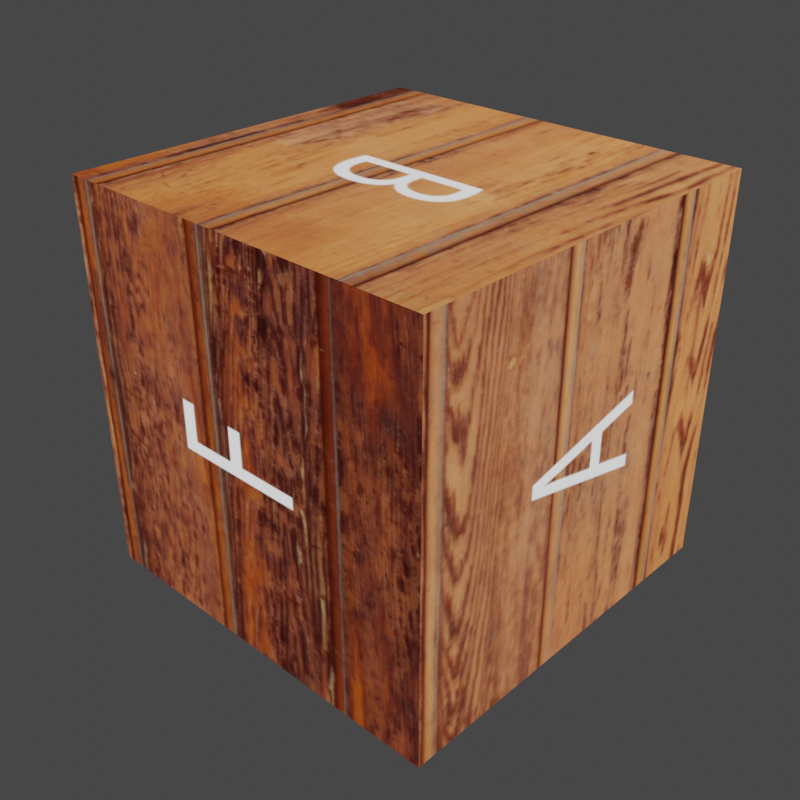
\includegraphics[width=\textwidth]{img/introduction/bad_uv_unwrapping_causes_seams.png}
%         \caption{Example of bad UV mapping which causes visible seams between the faces marked B-A and B-F.}
%         \label{fig:bad-uv-mapping}
%     \end{subfigure}
%     \hfill
%     \begin{subfigure}[t]{0.55\textwidth}
%         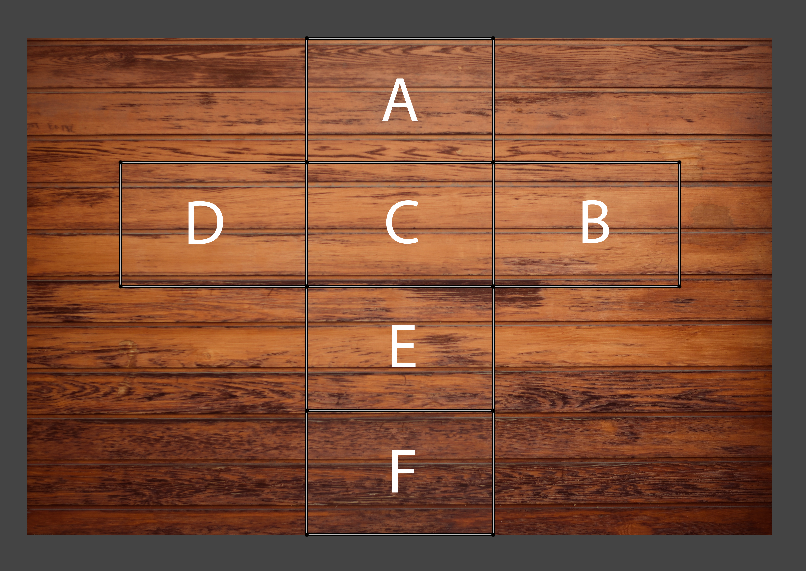
\includegraphics[width=\textwidth]{img/introduction/uv_unwrapping_blender.PNG}
%         \caption{UV unwrapping of the box.}
%         \label{fig:bad-uv-unwrapping}
%     \end{subfigure}
%     \caption{}
%     \label{}
% \end{figure}




